
\pdfbookmark{Основное содержание работы}{content}
\section*{Основное содержание работы}

\pdfbookmark[1]{Введение}{introduction}

\highlight{Во введении} обоснована актуальность темы исследования, показана степень ее разработанности, сформулированы цель и задачи работы, приведены научная новизна, теоретическая и практическая значимость, а также положения, выносимые на защиту.

\pdfbookmark[1]{Глава 1. Проблемы создания расчетных динамических моделей конструкций по результатам модальных испытаний}{partReview}

\highlight{В первой главе} выполнен обзор методов коррекции и ассемблирования расчетных моделей. Приведены основные теоретические сведения о методах классического и операционного модального анализа как источнике исходных данных для коррекции. Отмечено, что известные методы не всегда могут быть использованы для коррекции расчетных моделей летательных аппаратов.

\pdfbookmark[1]{Глава 2. Коррекция и синтез расчетных динамических моделей конструкций}{partModelUpdating}

\highlight{Вторая глава} посвящена разработке и развитию методик коррекции, освобождения и синтеза расчетных динамических моделей по результатам модальных испытаний. Математическая постановка задачи коррекции допускает изменение как упругих, так и диссипативных характеристик расчетной модели. Методика коррекции основывается на дополнении исходной конечно-элементной модели внутренними и внешними корректирующими элементами. Первые определяют изменение характеристик самой модели, а вторые отвечают за коррекцию параметров внешних связей, накладываемых на модель. Корректирующие элементы строятся на узлах исходной модели. 

Рассматривается конечно-элементная (КЭ) модель исследуемого объекта в виде матриц жесткости $ \mat{K} $ и масс $ \mat{M} $. Собственные числа $ \lambda $ и формы колебаний $ \mat{Y} $ определяются из решения обобщённой проблемы собственных значений.

Обладая конструкторской документацией и результатами контроля весов и моментов инерции деталей и агрегатов конструкции, инерционные характеристики модели могут быть определены достаточно точно. Но уточнение упругих характеристик модели не столь однозначно в силу совокупного объема факторов, обуславливающих погрешности моделирования: дискретизация модели, неточность задания упругих свойств материалов и граничных условий. Поэтому изменения вносятся только в матрицу жесткости путем добавления к исходной матрице $ \mat{K} $ матрицы жесткости корректирующей КЭ-модели $ \Delta \mat{K} $. Последняя записывается в виде суммы матриц жесткости внутренних $ \Delta \internal{\mat{K}} $ и внешних $ \Delta \external{\mat{K}} $ корректирующих элементов. Заметим, что жесткости корректирующих элементов могут быть отрицательными для изменения упругости конструкции в сторону уменьшения.

Матрица жесткости внутреннего корректирующего элемента в общем случае имеет вид:
\begin{equation}
	\Delta \internal{\mat{K}}_j = \sum\limits_{p\,=\,1}^{q} \internal{c}_{j+p-1} \mat{G}_j^{(p)}, \ j = 1 \hdots e, \label{eq:internalStiffMatrix}
\end{equation}
где $ \internal{c}_{j+p-1} $~---~неизвестная внутренняя корректирующая жесткость; $ q $~---~число внутренних корректирующих жесткостей, описывающих элемент; $ \mat{G}_j^{(p)} $~---~матрица внутреннего корректирующего элемента, составленная из длин и направляющих косинусов; $ e $~---~число внутренних корректирующих элементов. 

Число корректирующих жесткостей $ q $ зависит от числа физических параметров, которыми описывается добавляемый элемент. Для коррекции модели, составленной из объемных элементов, в качестве корректирующей КЭ-модели используется ферменная конструкция ($ q = 1 $). В случае, если динамические свойства модели существенно зависят от изгибных и крутильных жесткостей её балочных или оболочечных элементов, предлагается использовать корректирующую КЭ-модель из балочных элементов ($ q = 4 $). Матрицы корректирующего элемента имеют вид:
\begin{equation*}
	\begin{gathered}
	\mat{G}_j^{(1)} =
	\begin{pmatrix}
		\mat{D}_1 & \mat{0} & -\mat{D}_1 & \mat{0} \\
		\mat{0} & \mat{0} & \mat{0} & \mat{0} \\
		-\mat{D}_1 & \mat{0} & \mat{D}_1 & \mat{0} \\
		\mat{0} & \mat{0} & \mat{0} & \mat{0} \\
	\end{pmatrix},
	\mat{G}_j^{(2)} =
	\begin{pmatrix}
		6 \mat{D}_2 & 3 \ell \mat{D}_4 & -6 \mat{D}_2 & 3 \ell \mat{D}_4 \\
		3 \ell \trans{\mat{D}}_4 & 2 \ell ^ 2 \mat{D}_3 & -3 \ell \trans{\mat{D}}_4 & \ell ^ 2 \mat{D}_3 \\
		-6 \trans{\mat{D}}_2 & -3 \ell \mat{D}_4 & 6 \mat{D}_2 & -3 \ell \mat{D}_4 \\
		3 \ell \trans{\mat{D}}_4 & \ell ^ 2 \trans{\mat{D}}_3 & -3 \ell \trans{\mat{D}}_4 & 2 \ell ^ 2 \mat{D}_3
	\end{pmatrix}, \\
	\mat{G}_j^{(3)} =
	\begin{pmatrix}
		6 \mat{D}_3 & -3 \ell \trans{\mat{D}}_4 & -6 \mat{D}_3 & -3 \ell \trans{\mat{D}}_4 \\
		-3 \ell \mat{D}_4 & 2 \ell ^ 2 \mat{D}_2 & 3 \ell \mat{D}_4 & \ell ^ 2 \mat{D}_2 \\
		-6 \trans{\mat{D}}_3 & 3 \ell \trans{\mat{D}}_4 & 6 \mat{D}_3 & 3 \ell \trans{\mat{D}}_4 \\
		-3 \ell \mat{D}_4 & \ell ^ 2 \trans{\mat{D}}_2 & 3 \ell \mat{D}_4 & 2 \ell ^ 2 \mat{D}_2
	\end{pmatrix},
	\mat{G}_j^{(4)} =
	\begin{pmatrix}
		\mat{0} & \mat{0} & \mat{0} & \mat{0} \\
		\mat{0} & \mat{D}_1 & \mat{0} & -\mat{D}_1 \\
		\mat{0} & \mat{0} & \mat{0} & \mat{0} \\
		\mat{0} & -\mat{D}_1 & \mat{0} & \mat{D}_1 \\
	\end{pmatrix},
	\end{gathered}
\end{equation*}
где $ \ell $~---~длина корректирующего балочного элемента; $ \mat{D}_1, \mat{D}_2, \mat{D}_3, \mat{D}_4 $~---~матрицы, состоящие из направляющих косинусов.

В качестве внешних корректирующих элементов используются пружинные опоры, прикрепленные к неподвижному основанию. Матрица $ \Delta \external{\mat{K}} $ имеет следующий вид:
\begin{equation}
	\Delta \external{\mat{K}} = \operatorname{diag} \cbrackets{\external{c}_1, \external{c}_2, \hdots, \external{c}_N}, \label{eq:externalStiffMatrix}
\end{equation}
где $ N $~---~размерность КЭ-модели, $ \external{\mat{c}} $~---~неизвестные внешние корректирующие жесткости. 

Рассматривается итерационный алгоритм коррекции, позволяющий избежать построения прямых функциональных зависимостей, которые сопряжены с существенной вычислительной трудоемкостью многократного решения обобщенной проблемы собственных значений. На каждом шаге коррекции жесткости корректирующих элементов являются неизвестными параметрами $ \mat{c} = \rbrackets{\internal{\mat{c}}, \external{\mat{c}}} $, которые определяются из решения задачи безусловной минимизации целевой функции:
\begin{gather}
	\sum\limits_{i = 1} ^ s w_i \sbrackets{\trans{\rbrackets{\mat{Y}_i ^ {(j)}}} \Delta \mat{K} ^ {(j + 1)} \mat{Y}_i ^ {(j)} - \Delta \lambda_i ^ {(j + 1) \ast} \trans{\rbrackets{\mat{Y}_i ^ {(j)}}} \mat{M} \mat{Y}_i ^ {(j)}} ^ 2 \rightarrow \min_{\mat{c}},
\end{gather}
где $ s $~---~число корректируемых тонов; $ j $~---~номер итерации; $ \Delta \lambda_i ^ {\ast}$~---~разница между текущими и целевыми (экспериментальными) собственными значениями $ i $-го тона; $ w_i $~---~весовой коэффициент, определяющий значимость $ i $-го тона.

Для решения задачи минимизации целевой функции применяется метод сопряженных градиентов. Используются аналитические выражения для компонент вектора-градиента целевой функции, что позволяет кратно сократить время для осуществления коррекции.

На рисунке~\ref{fig:principalSchemeUpdating} приведена принципиальная схема, иллюстрирующая физическую сторону предлагаемой методики на примере простой модели летательного аппарата. В данном случае модель составлена из объемных и оболочечных элементов, поэтому для изменения её динамических свойств вводятся как ферменные, так и балочные корректирующие элементы. Кроме того, для описания модели упругого основания, вводятся пружинные элементы. Таким образом, корректирующая модель является <<каркасной структурой>> исходной модели.

\begin{figure}[H]
	\hfill
	\begin{tikzpicture}[scale = 1]
		\pgfmathsetmacro{\nodeDist}{0.1}
		\pgfmathsetmacro{\shiftText}{0.0}
		% Исходная модель
		\node[inner sep = 0pt] (initial) at (0, 0) {\includegraphics[width = 0.32\textwidth]{simple-model-initial}};
		\node[inner sep = 0pt, below = \shiftText of initial.south] (textInitial) {Исходная модель};
		% Знак
		\node [font = \fontsize{42}{44}, below = \nodeDist of textInitial.south, color = blue] (sumSign) {\bfseries +};
		% Коррректирующие элементы
		\node[inner sep = 0pt, below = -\nodeDist of sumSign.south] (elements) {\includegraphics[width = 0.32\textwidth]{simple-model-elements}};
		\node[inner sep = 0pt, below = \shiftText of elements.south] (textElements) {Корректирующие элементы};
		% Скорректированная модель
		\draw (sumSign.east) ++ (3.5, 0) node [right] (updated) {\includegraphics[width = 0.5\textwidth]{simple-model-updated}};
		\draw [line width = 1.5mm, -{Latex[length = 8mm]}, color = red](sumSign.east) ++ (2.5, 0) --++ (2, 0);
		\node[inner sep = 0pt, below = \shiftText of updated.south] (textUpdated) {Скорректированная модель};
	\end{tikzpicture}
	\caption{Принципиальная схема коррекции} \label{fig:principalSchemeUpdating}
\end{figure}

Набор корректирующих элементов формируется автоматически на основе портрета матрицы жесткости корректируемой модели. В общем случае число таких корректирующих элементов определяется количеством связей между степенями свободы узлов в матрице, но оно может быть сокращено посредством выбора областей коррекции, например, элементов конструкции с наибольшей неопределенностью физических и геометрических характеристик. 

Экспериментальные исследования показали, что обычно в окрестности частот фазового резонанса монофазные колебания совпадают с собственными. Это означает, что матрица демпфирования в главных координатах имеет диагональный вид: $ \operatorname{diag} \cbrackets{h_1 ^ \ast, \hdots, h_i ^ \ast, \hdots, h_s ^ \ast} $, где $ h_i ^ \ast $~---~обобщенный коэффициент демпфирования i-го тона. Матрица демпфирования в физической системе координат строится в два этапа: в качестве нулевого приближения используется гипотеза Е.\,С.~Сорокина, а затем для достижения целевых обобщенных коэффициентов демпфирования вводятся корректирующие элементы.

Нулевое приближение матрицы демпфирования записывается в виде:
\begin{equation}
	\mat{H} = \alpha \mat{K} ^ \ast + \beta \mat{M},
\end{equation}
где $ \mat{K} ^ \ast $~---~матрица жесткости после коррекции, $ \alpha, \beta $~---~постоянные коэффициенты.

Частоты и формы собственных колебаний, вычисленные в результате решения обобщенной проблемы, остаются неизменными в процессе восстановления матрицы демпфирования. Обобщенные жесткости $ \kappa_i $ и массы $ \mu_i $ корректируемых тонов колебаний используются для определения коэффициентов $ \alpha $ и $ \beta $ в результате решения задачи минимизации целевой функции:
\begin{equation}
	\sum \limits_{i\,=\,1} ^ s w_i \left( 1 - \frac{\alpha \kappa_i + \beta \mu_i}{h_i ^ \ast} \right)^2 \rightarrow \min_{\alpha, \beta}.
\end{equation}

По аналогии с~\eqref{eq:internalStiffMatrix} и \eqref{eq:externalStiffMatrix} нулевое приближение матрицы демпфирования уточняется введением корректирующих элементов:
\begin{equation}
	\tilde{\mat{H}}(\eta_1, \eta_2, ..., \eta_m) = \mat{H} + \Delta \internal{\mat{H}} + \Delta \external{\mat{H}},
\end{equation}
где $ \Delta \internal{\mat{H}} $ и $ \Delta \external{\mat{H}} $~---~матрицы демпфирования внутренних и внешних корректирующих элементов, а параметры $ \mat{\eta} $ вводятся аналогично корректирующим коэффициентам $ \mat{c} $. Под внутренним демпфированием понимаются потери механической энергии за счет трения в материалах модели, а под внешним~---~рассеяние энергии при взаимодействии модели с окружающей средой, например, воздухом. Последнее особенно актуально для крупногабаритных конструкций.

Алгоритм восстановления матрицы демпфирования заключается в том, чтобы найти такие параметры $ \mat{\eta} $, которые будут решением следующей недоопределенной системы уравнений:
\begin{equation}
	f_i = \trans{\rbrackets{\mat{Y}_i ^ \ast}} \tilde{\mat{H}} \mat{Y}_i ^ \ast - h_i ^ \ast, \ i = 1 \hdots s. \label{eq:systemDampUpdating}
\end{equation}

Решением системы~\eqref{eq:systemDampUpdating} считается решение задачи безусловной минимизации целевой функции, равной сумме квадратов каждого из уравнений с взвешенной суммой квадратов коэффициентов демпфирования:
\begin{equation}
	\sum \limits_{i\,=\,1} ^ s w_i f_i ^ 2 + w_c \sum \limits_{i\,=\,1}^s \eta_i ^ 2 \rightarrow \min_\mat{\eta},
	\label{eq:objFinalDampFunUpdating}
\end{equation}
где $ w_c $~---~параметр регуляризации.

Важно отметить, что расчетная модель летательного свободна от закреплений. В то же время для модальных испытаний авиационная техника либо устанавливается на шасси, либо помещается на специальную систему упругого вывешивания, а космические конструкции~---~на систему обезвешивания. Системы упругого вывешивания и обезвешивания, влияние которых на свободную конструкцию строго регламентировано, являются сложными и дорогостоящими техническими сооружениями. Поэтому разработана методика освобождения скорректированной КЭ-модели от связей, соответствующих условиям проведения эксперимента. 

Суть методики освобождения заключается в том, что матрицы жесткости и масс расширяются шестью степенями свободы $ \mat{\xi} $, которые отвечают за перемещения и повороты модели как жесткого целого. Дополнительные элементы матриц рассчитываются следующим образом:
\begin{equation}
	\begin{pmatrix}
		\mat{K} & -\trans{\rbrackets{\sum \mat{k}}} \\
		 -\sum \mat{k} & \kappa + \sum \sum \mat{k}
	\end{pmatrix}
	\begin{Bmatrix}
		\tilde{\mat{Y}} \\
		\xi
	\end{Bmatrix}
	+
	\begin{pmatrix}
		\mat{M} & \mat{0} \\
		\mat{0} & \mu - \sum \sum \mat{m}
	\end{pmatrix}
		\begin{Bmatrix}
		\ddot{\tilde{\mat{Y}}} \\
		\ddot{\xi}
	\end{Bmatrix}
	= 0,
\end{equation}
где $ \sum \mat{k} \in \set{R}^{6 \times n}$, $ \sum \mat{m} \in \set{R}^{6 \times n}$, $ \sum \sum \mat{m} \in \set{R}^{6 \times 6} $~---~дополнительные матричные элементы; $ \tilde{\mat{Y}} $~---~вектор узловых перемещений относительно некоторой точки, например, центра тяжести.

С целью оценки устойчивости результата коррекции к погрешностям в значениях частот, определенных экспериментально, использован метод статистического моделирования. Суть метода состоит во внесении случайных отклонений в исходные значения частот собственных колебаний с последующей оценкой искажений форм колебаний по критерию модального соответствия~$ \varepsilon_{\mathrm{MAC}} $. Для моделирования ошибок $\Delta \mat{f} $ используется генератор случайных чисел, имеющих усеченное нормальное распределение. Концы этого распределения совмещены с предельным шумовым уровнем и соответствуют утроенному среднеквадратическому отклонению. 

На примере свободной прямоугольной пластины показаны зависимости искажений форм колебаний относительно ошибок в целевых частотах, полученные при разном числе корректируемых тонов собственных колебаний~\figref{fig:perturbation-plate-errors}. При этом точки, составляющие эти зависимости, определены путем многократного проведения независимых испытаний (коррекций) на одном уровне шума. Число этих испытаний $ N_\Sigma $, которое потребовалось для стабилизации величины центрального момента критерия модального соответствия, приведено на рисунке~\ref{fig:perturbation-plate-samplesize}. Установлено, что методика устойчива во всем диапазоне вносимых отклонений. Более того, при увеличении числа тонов кривые стремятся к предельной огибающей. Аналогичный результат получен для более сложной конструкции~---~модели космического аппарата (КА).

\vspace{-1em}
\begin{figure}[!htb]
	\centering
	\begin{minipage}[b]{0.49\textwidth}
		\centering
		\begin{tikzpicture}[scale = 1]
			\begin{semilogyaxis}[
				xlabel           = {$\Delta \mat{f} $, \% },
				ylabel           = {$ \varepsilon_{\mathrm{MAC}} $, \%},
				ylabel shift     = -5 pt,
				grid             = major,
				legend columns   = 2,
				legend style     = {
					at           = {(0.81, 0.03)},
					anchor       = south,
					fill         = white,
					fill opacity = 0.6,
					draw opacity = 1,
					text opacity = 1,
				},
				ylabel near ticks,  
				xtick            = {0, 1, 2, 3, 4, 5},
				ytick            = {1e-6, 1e-4, 1e-2, 1e0},
				mark size        = 1.5pt,
				width            = 8.75cm
			]
				\pgfplotstableread{images/partModelUpdating/perturbation-plate-errors.txt}\contentFile
				\addplot[color = blue, mark = *] table [x index = 0, y index = 1] {\contentFile};
				\addplot[color = red, mark = triangle*] table [x index = 0, y index = 2] {\contentFile};
				\addplot[color = olive, mark = diamond*] table [x index = 0, y index = 3] {\contentFile};
				\addplot[color = purple, mark = halfcircle*] table [x index = 0, y index = 4] {\contentFile};
				\addplot[color = teal, mark = x] table [x index = 0, y index = 5] {\contentFile};
				\legend{$ 1 $, $ 3 $, $ 5 $, $ 7 $, $ 9 $}
			\end{semilogyaxis}
		\end{tikzpicture}
		\caption{Погрешность определения форм колебаний свободной пластины} \label{fig:perturbation-plate-errors}
	\end{minipage}
	\hfill
	\begin{minipage}[b]{0.49\textwidth}
		\centering
		\begin{tikzpicture}[scale = 1]
			\begin{axis}[
				xlabel           = {$\Delta \mat{f} $, \% },
				ylabel           = {$ N_\Sigma $},
				ylabel shift     = -10 pt,
				legend columns   = 1,
				legend style     = {
					at           = {(0.03, 0.72)},
					anchor       = west,
					fill         = white,
					fill opacity = 0.6,
					draw opacity = 1,
					text opacity = 1,
				},
				ylabel near ticks,
				try min ticks = 6,
				bar width  = 3pt,
				width      = 8.75cm,
				ybar stacked,
				scaled y ticks = base 10:-3,
	          	xmin = 0.15, xmax = 5.05, ymin = 0
			]
				\pgfplotstableread{images/partModelUpdating/perturbation-plate-samplesize.txt}\contentFile
				\addplot table [x index = 0, y index = 1] {\contentFile};
				\addplot table [x index = 0, y index = 2] {\contentFile};
				\addplot table [x index = 0, y index = 3] {\contentFile};
				\addplot table [x index = 0, y index = 4] {\contentFile};
				\addplot table [x index = 0, y index = 5] {\contentFile};
				\legend{$ 1 $, $ 3 $, $ 5 $, $ 7 $, $ 9 $}
			\end{axis}
		\end{tikzpicture}
		\caption{Число независимых испытаний свободной пластины} \label{fig:perturbation-plate-samplesize}
	\end{minipage}
\end{figure}

Развита методика, состоящая в декомпозиции крупногабаритных трансформируемых конструкций (КТК) на составные части, которые подвергаются модальным испытаниям независимо друг от друга. Результаты испытаний используются для коррекции, освобождения и синтеза расчетных моделей составных частей~\figref{fig:schemeDecomposition}. Обоснован выбор граничных условий в испытаниях составных частей. Кроме того, имея в виду достижение физической согласованности расчетных моделей, предложено использовать для коррекции результаты нескольких экспериментов при различных условиях закрепления одной составной части.

\begin{figure}[!htb]
	\centering
	\begin{subfigure}[b]{0.54\textwidth}
		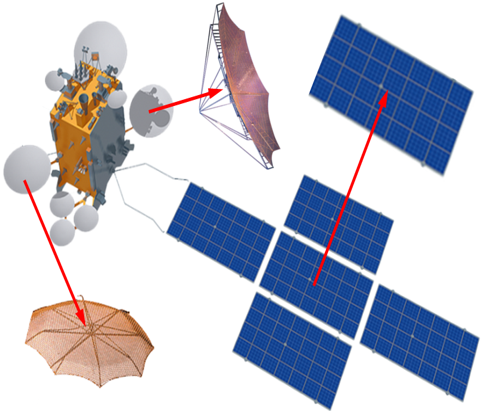
\includegraphics[width = \textwidth]{images/synopsis/decomposition}
	\end{subfigure}
	\hfill
	\begin{subfigure}[b]{0.45\textwidth}
	     % Определение стиля
        \tikzstyle{blockWide} = [rectangle, draw = black, fill = blue!15, rounded corners, text width = 20em, text centered, minimum height = 1.5em, drop shadow] 
        \tikzstyle{blockWideC} = [blockWide, fill = red!20]
        \tikzstyle{arrow} = [draw, very thick, color = black!90, line width = 0.6mm, -latex'] 
        \small
        % Задание перменных
        \def\nodeDist{0.45cm}
        % Отрисовка блок-схемы
        \begin{tikzpicture}[scale = 1, transform shape]
            % Задание узлов		
            \node (modalTests) [blockWide] {Модальные испытания \\ составных частей конструкции};
            \node (modelUpdating) [blockWide, below = \nodeDist of modalTests] {Коррекция расчетных моделей \\ составных частей  конструкции \\ по результатам испытаний};
            \node (checkInfluence) [blockWide, below = \nodeDist of modelUpdating] {Освобождение расчетных моделей \\ составных частей конструкции};
            \node (buildRealModel) [blockWide, below = \nodeDist of checkInfluence] {Синтез расчетной модели полной \\ конструкции из её составных частей};
            \node (buildMathModel) [blockWide, below = \nodeDist of buildRealModel] {Определение динамических \\ характеристик полной расчетной модели};
            % Соединение узлов
            \draw [arrow] (modalTests.south) -- (modelUpdating.north);
            \draw [arrow] (modelUpdating.south) -- (checkInfluence.north);
            \draw [arrow] (checkInfluence.south) -- (buildRealModel.north);
            \draw [arrow] (buildRealModel.south) -- (buildMathModel.north);
        \end{tikzpicture}
	\end{subfigure}
    \caption{Схема методики синтеза расчетных моделей КТК} \label{fig:schemeDecomposition}
\end{figure}  

Методика синтеза протестирована на примере модели космического аппарата, состоящего из орбитального модуля и панелей солнечных батарей. Модели каждой составной части корректировались по девяти частотам собственных колебаний, используя данных двух виртуальных экспериментов. Распределение изменений узловых жесткостей по всем линейным степеням свободы для моделей составных частей после коррекции показано на рисунке~\ref{fig:test-spacecraft-distribution}. Максимальная погрешность в определении первых шестнадцати частот синтезированной (глобальной) модели до коррекции равнялась $ 5.1 $ \%, а после коррекции составила $ 0.1 $ \%~\tabref{tab:resultUpdatingTestSpacecraft}. 
\vspace{-0.5em}
\begin{figure}[H]
	\centering
	\begin{subfigure}[t]{0.41\textwidth}
		\centering
		\includegraphics[width = \textwidth]{test-spacecraft-orbital-distribution}
		\caption{Орбитальный модуль} \label{subfig:test-orbital-distribution}
	\end{subfigure}
	\qquad
	\begin{subfigure}[t]{0.39\textwidth}
		\centering
		\includegraphics[height = \textwidth]{test-spacecraft-panel-distribution}
		\caption{Панели солнечных батарей} \label{subfig:test-panel-distribution}
	\end{subfigure}
	\vspace{0.7em}
	\caption{Изменения жесткостей при коррекции моделей составных частей} \label{fig:test-spacecraft-distribution} 
\end{figure}

\begin{figure}[!htb]
	\centering
	\begin{minipage}{0.52\textwidth}
		\hspace{2em} Сходимость алгоритма коррекции оценивалась по частотному критерию $ \lVert \mat{\alpha} \rVert_{\max} $, равному наибольшему относительному отклонению расчетных частот от целевых значений~\figref{fig:test-spacecraft-convergence}.
		\vspace{-1.5em}
		\begin{center}
			\begin{tikzpicture}[scale = 1]
				\begin{semilogyaxis}[
					xlabel            = {Номер итерации коррекции},
					ylabel            = {$ \lVert \mat{\alpha} \rVert_{\max} $}, 
					ylabel shift      = -5 pt,
					width             = 9cm,
					grid              = both,
					legend cell align = left,
					legend style      = {
						at            = {(0.02, 0.12)},
						anchor        = west,
						fill          = white,
						fill opacity  = 0.6,
						draw opacity  = 1,
						text opacity  = 1,
					},
					ylabel near ticks,
					xmin = 0, xmax = 8
				]
					\addplot table {images/partModelUpdating/test-spacecraft-panels-convergence.txt};
					\addplot table {images/partModelUpdating/test-spacecraft-orbital-convergence.txt};
					\legend{Панели солнечных батарей, Орбитальный модуль}
				\end{semilogyaxis}
			\end{tikzpicture}
			\caption{Оценка сходимости коррекции} \label{fig:test-spacecraft-convergence}
		\end{center}
	\end{minipage}
	\hfill
	\begin{minipage}{0.45\textwidth}
		\centering
		\vspace{0.1em}
		\begin{talltblr}[
			caption = {Cинтез модели КА},
			label = {tab:resultUpdatingTestSpacecraft}
		]{
			colspec = {|X[c, -1]|X[c]|X[c]|X[c]|X[c]|},
			hlines,
			colsep = 1pt,
			rows = {font = \small}
		}
			\SetCell[r = 3]{c} Тон & \SetCell[c = 4]{c} Погрешность в частотах, \% &&& \\
			& \SetCell[r = 2]{c} Исходная & \SetCell[c = 3]{c} Коррекция по девяти частотам && \\
			& & Панелей & Модуля & {Панелей \\ и модуля} \\ \hline
			7 & -4.689 & -2.120 & -2.756 & -0.021 \\
			8 & -4.678 & -2.078 & -2.782 & -0.018 \\
			9 & -5.121 & -4.447 & -0.674 & 0.100  \\
			10 & -5.040 & -4.760 & -0.354 & -0.028 \\
			11 & -5.040 & -4.760 & -0.357 & -0.032 \\
			12 & -5.121 & -4.443 & -0.687 & 0.091 \\
			13 & -4.102 & -0.966 & -3.161 & 0.011 \\
			14 & -4.112 & -0.999 & -3.135 & 0.016 \\
			15 & -3.303 & -0.234 & -3.066 & -0.006 \\
			16 & -3.303 & -0.234 & -3.066 & -0.005 \\
		\end{talltblr}
	\end{minipage}
	\vspace{0.3em}
\end{figure}

\vspace{-0.5em}

\begin{wrapfigure}[17]{r}{0.6\textwidth}
	\centering
	\vspace{-0.3em}
	\includegraphics[width = 1\linewidth]{gencalc-interface}
	\caption{Определение модальных параметров} \label{fig:gencalc-interface}
\end{wrapfigure}

\pdfbookmark[1]{Глава 3. Результаты модальных испытаний как исходные данные для коррекции расчетных моделей конструкций}{partModalAnalysis}

\highlight{В третьей главе} развиты методы классического и операционного модального анализа, позволяющие получать достоверные оценки динамических параметров для коррекции. С целью обеспечения возможности оперативного расчета обобщенных характеристик в ходе модальных испытаний, составлена программная реализация, позволяющая посредством графического интерфейса~\figref{fig:gencalc-interface} варьировать параметры расчета и исследовать зависимости получаемых характеристик несколькими способами одновременно. 

Одним из ключевых требований обеспечения непрерывности производственного процесса авиационной техники является сокращение времени между натурными испытаниями и первым вылетом. Этой цели служит разработанная программа~\figref{fig:analyzer-interface}, использующая программный интерфейс \name{Testlab Automation} для обработки и представления результатов модального анализа непосредственно в процессе испытаний.

\begin{wrapfigure}[15]{r}{0.6\textwidth}
	\centering
	\includegraphics[width = \linewidth]{analyzer-interface}
	\caption{Экспресс-представление результатов} \label{fig:analyzer-interface}
\end{wrapfigure}

Изложена методика контроля зазоров в технических изделиях по искажениям портретов вынужденных колебаний в процессе вибрационных испытаний. Представлен способ поэтапного выявления всех зазоров в объекте испытаний, которые приводят к искажениям портретов колебаний. В рамках описываемого подхода разработана и интегрирована в программное обеспечение управления испытаниями программа анализа портретов колебаний. Методика обнаружения дефектов по искажениям портретов колебаний использована для диагностирования самолётов в процессе модальных испытаний~\figref{fig:distortion-wiring-backlash}, а также космических аппаратов открытого исполнения в технологических вибрационных испытаниях~\figref{fig:distortion-spacecraft}. 

\vspace{-0.3em}

\begin{figure}[!htb]
	\centering
	\begin{minipage}{0.59\textwidth}
		\centering
		\includegraphics[width = \linewidth]{distortion-wiring-backlash} 
		\captionof{figure}{Люфт в соединении ручки управления с проводкой} \label{fig:distortion-wiring-backlash}
	\end{minipage}
	\hfill
	\begin{minipage}{0.4\textwidth}
		\centering
		\includegraphics[width = 0.8\linewidth]{distortion-spacecraft}
		\captionof{figure}{Зазоры в узлах установки солнечных батарей} \label{fig:distortion-spacecraft}
	\end{minipage}
	\vspace{0.5em}
\end{figure}

\begin{wrapfigure}[10]{r}{0.5\textwidth}
	\begin{center}
		\vspace{-1.4em}
		\includegraphics[width = 1\linewidth]{reflector-experiment}
		\caption{Испытания рефлектора КА} \label{fig:reflector-experiment}
	\end{center}
\end{wrapfigure}

\vspace{-0.2em}

Разработан способ определения модальных параметров, обладающий низкий чувствительностью к дрейфу показаний (тренду) акселерометров, регистрирующих отклики конструкции на импульсное воздействие (\name{ADA}). При этом разметка по времени анализируемых участков осуществляется автоматически методом сегментации. Методы операционного модального анализа: \name{SSI}, \name{ERA}, \name{N4SID} и \name{ADA}, протестированы на примере имитационной модели беспилотного летательного аппарата и применены для определения модальных характеристик рефлектора КА по результатам испытаний в акустической камере~\figref{fig:reflector-experiment}. Исследована устойчивость значений определяемых модальных характеристик в зависимости от продолжительности записи и частоты дискретизации сигналов.

\begin{wrapfigure}[15]{r}{0.5\textwidth}
	\begin{center}
		\vspace{-2em}
		\hspace{-1em}
		\begin{tikzpicture}[scale = 1]
			\small
			\begin{axis}[
				xlabel            = {$ v $, км/ч},
				ylabel            = {$ \delta $},
				ylabel shift      = -2 pt,
				y dir             = reverse,
				grid              = major,
				legend columns    = 1,
				legend cell align = {left},
				legend style      = {
					at            = {(0.025, 0.76)},
					anchor        = west,
					fill          = white,
					fill opacity  = 0.6,
					draw opacity  = 1,
					text opacity  = 1,
				},
				ylabel near ticks,
				ymin = 0,
				x tick label style = {
					/pgf/number format/.cd,
					set thousands separator = {},
					fixed
				},
				y tick label style = {
					/pgf/number format/.cd,
					fixed
				},
				ylabel near ticks,  
				try min ticks    = 6,
				mark size        = 1.25pt,
				width            = 9cm,
				height           = 8.25cm,
			]
				\pgfplotstableread{images/synopsis/flight-decrements-2.txt}\contentFile
				\addplot[color = blue, thick, mark = *, smooth, tension = 0.2] table [x index = 0, y index = 1] {\contentFile};
				\addplot[color = gray, thick, mark = triangle*, smooth, tension = 0.2] table [x index = 0, y index = 2] {\contentFile};
				\addplot[color = teal, thick, mark = diamond*, smooth, tension = 0.2] table [x index = 0, y index = 3] {\contentFile};
				\addplot[color = red, thick,  mark = halfcircle*, smooth, tension = 0.2] table [x index = 0, y index = 4] {\contentFile};
				\addplot[color = orange, thick, densely dashed, mark = o, mark options = {solid}, smooth, tension = 0.2] table [x index = 0, y index = 5] {\contentFile};
				\addplot[color = violet, thick, densely dashed, mark = o, mark options = {solid}, smooth, tension = 0.2] table [x index = 0, y index = 6] {\contentFile};
				\legend{\name{SSI-DD}, \name{ERA}, \name{ADA}, \name{N4SID}, {\name{ЛИИ}, оценка сверху}, {\name{ЛИИ}, оценка снизу}}
			\end{axis}
		\end{tikzpicture}
		\caption{Скоростные зависимости логарифмического декремента} \label{fig:flight-decrements}
	\end{center}
\end{wrapfigure}

Получены оценки динамических параметров по результатам летных испытаний в ходе которых записывались отклики на управляемое внешнее воздействие при полете самолёта на разных скоростных режимах $ v $. Определенные после обработки и обобщения значения частот и логарифмических декрементов $ \delta $~\figref{fig:flight-decrements} являются исходными данными для исследования аэроупругой устойчивости. Для оценки корректности обработки проведено сопоставление результатов с данными летно-исследовательского института имени М.\,М.~Громова~(ЛИИ). 

\pdfbookmark[1]{Глава 4. Решение практических задач коррекции расчетных моделей}{partAprobation}

\highlight{Четвертая глава} посвящена применению разработанных методик для решения практических задач коррекции, освобождения и синтеза расчетных динамических моделей. Разработан способ моделирования податливости закреплений в условиях эксперимента. 

\begin{wrapfigure}[22]{r}{0.5\textwidth}
	\begin{center}
		\vspace{-3em}
		\includegraphics[width = 1\linewidth]{tu-204-experiment}
		\caption{Общий вид ДПМ} \label{fig:tu-204-experiment}
		\vspace{1em}
		\begin{talltblr}[
			caption = {Результаты коррекции ДПМ},
			label   = {tab:updatingTu204}
		]{
			colspec = {|c|c|c|c|c|c|c|c|},
			hlines,
			colsep = 7pt,
			rows = {font = \small}
		}
			\SetCell[r = 3]{c} Тон & \SetCell[c = 7]{c} {Погрешность до и после коррекции, \%}  \\
			& \SetCell[r = 2]{c} До & \SetCell[c = 6]{c} После \\ 
			& & 1 & 2 & 3 & 4 & 5 & 6 \\ \hline
			1 & 1.5 & 0.0 & 0.0 & 0.0 & 0.0 & 0.0 & 0.0 \\
			2 & 1.7 & -0.6 & 0.0 & 0.0 & 0.0 & 0.0 & 0.0 \\
			3 & 5.3 & 4.7 & 4.7 & 0.0 & 0.0 & 0.0 & 0.0 \\ 
			4 & 4.2 & 3.5 & 3.3 & 2.6 & 0.0 & 0.0 & 0.0 \\
			5 & -1.8 & -4.4 & -3.2 & -3.9 & -4.4 & 0.0 & 0.0 \\
			6 & 4.2 & 3.7 & 3.8 & 3.4 & 2.0 & 3.3 & 0.0 \\
		\end{talltblr}
	\end{center}
\end{wrapfigure}

Методика коррекции апробирована на динамически-подобной модели (ДПМ) самолёта \mbox{Ту-204}, выполненной по отсечно-балочной схеме. Для проведения экспериментального модального анализа ДПМ была вывешена на упругой подвеске малой жесткости~\figref{fig:tu-204-experiment}. Средствами \name{Ansys} создана КЭ-модель, имеющая $ 752 $ тысячи степеней свободы. Коррекция КЭ-модели проводилась по шести наборам, состоящих из экспериментально определенных частот. Каждый последующий набор дополнял предыдущий одним тоном собственных колебаний. Итерационный процесс коррекции завершался при достижении целевых значений частот с точностью $0.0001$\,\%. Результаты коррекции сведены в таблице~\ref{tab:updatingTu204}.

Осуществлен синтез глобальной модели каркаса зонтичной антенны по результатам испытания её составных частей. Податливость закрепления одной из составных частей в ходе экспериментов смоделирована упругими элементами, параметры которых определены на основе данных дополнительных статических испытаний. В результате проведенных исследований показано, что использование полноразмерных моделей составных частей является предпочтительным по отношению к редуцированным моделям в силу того, что первые более полно описывает связи между подконструкциями. 

\begin{wrapfigure}[14]{r}{0.5\textwidth}
	\begin{center}
		\vspace{-3em}
		\includegraphics[width = \linewidth]{wing-experiment} 
		\captionof{figure}{Общий вид ОЧК} \label{fig:wing-experiment}
	\end{center}
\end{wrapfigure}

Выполнена коррекция расчетной модели отъемной части крыла (ОЧК) изделия \mbox{С-70}~\figref{fig:wing-experiment}. По результатам экспериментального модального анализа было выявлено, что полученные частоты собственных колебаний консоли крыла существенно отличаются от расчетных. Это во многом обусловлено тем, что масса конструкции, выполненной из композиционных материалов, в расчетной схеме представлялась дискретно, а жесткостное распределение моделировалось невесомыми панелями с изотропными характеристиками.  Однако, даже в случае столь существенных различий в схематизации, целевые частоты по пяти тонам собственных колебаний были достигнуты с заданной точностью. 

\begin{wrapfigure}[13]{r}{0.5\textwidth}
	\begin{center}
		\vspace{-1.25em}
		\includegraphics[width = \linewidth]{girder-full-system} 
		\captionof{figure}{Гирдер с оборудованием} \label{fig:girder-experiment}
	\end{center}
\end{wrapfigure}

Уточнены упругие характеристики модели гирдера (подставки), который используется для размещения электрофизического оборудования в накопительной части кольца центра коллективного пользования <<Сибирский кольцевой источник фотонов>>~\figref{fig:girder-experiment}. Коррекция позволит улучшить эксплутационные характеристики совместной системы гирдера с оборудованием за счет избежания возникновения резонансов от сейсмических колебаний, приводящих к потере качества электронного пучка. По результатам экспериментальных исследований установлено, что формы собственных колебаний, соответствующие низшим тонам, происходят при совместном перемещении гирдера и блока фундамента, на который опираются регулируемые опоры. Поэтому построена модель фундамента, идентифицированная по пяти частотам собственных колебаний, соответствующих этим движениям. Затем модель гирдера на упругом основании скорректирована по шести частотам упругих тонов собственных колебаний. Наибольшие изменения узловых жесткостей достигались в местах сопряжения конструктивных элементов гирдера. Длительность коррекции расчетной модели гирдера, обладающей $ 304 $ тысячами степеней свободы, составила $ 14 $~минут. Результаты коррекции сведены в таблице~\ref{tab:girder-results}. Минимальный критерий модального соответствия, связывающий формы колебания до и после коррекции, составил $ 0.941 $~\figref{fig:girder-mac}. Суммарные модальные эффективные массы корректируемых тонов колебаний по направлениям глобальной системы координат составили: $ 79 $, $ 96 $ и $ 97 $ \%. 

\begin{figure}[!htb]
	\centering
	\begin{minipage}{0.49\textwidth}
		\begin{talltblr}[
			caption = {Коррекция модели гирдера}, 
			label = {tab:girder-results}
		]{
			colspec = {|X[c, -1]|X[c, 1.3]|X[c]|X[c]|X[c]|}, 
			hlines,
			colsep = 1pt,
			rows = {font = \small}
		}
			\SetCell[r = 2]{c} Тон & \SetCell[c = 2]{c} Частота, Гц && \SetCell[c = 2]{c} {Погрешность до и \\ после коррекции, \%} \\
			& Эксперимент & Исходная модель & До & После \\ \hline
			6 & 119.51 & 135.08 & 13.03 & \SetCell[r = 6]{c} 0.00 \\
			7 & 140.97 & 146.46 & 3.89 &  \\
			8 & 148.13 & 160.07 & 8.06 &  \\
			9 & 189.65 & 210.48 & 10.98 & \\
			10 & 197.53 & 214.18 & 8.43 & \\
			11 & 242.24 & 253.51 & 4.65 & \\
		\end{talltblr}
	\end{minipage}
	\hfill
	\begin{minipage}{0.5\textwidth}
		\centering
		\includegraphics[width = \linewidth]{girder-mac-scaled}
		\captionof{figure}{Сравнение форм колебаний} \label{fig:girder-mac}
	\end{minipage}
\end{figure}